%%%%%%%%%%%%%%%%%%%%%%%%%%%%%%%%%%%%%%%%%
% Arsclassica Article
% LaTeX Template
% Version 1.1 (10/6/14)
%
% This template has been downloaded from:
% http://www.LaTeXTemplates.com
%
% Original author:
% Lorenzo Pantieri (http://www.lorenzopantieri.net) with extensive modifications by:
% Vel (vel@latextemplates.com)
%
% License:
% CC BY-NC-SA 3.0 (http://creativecommons.org/licenses/by-nc-sa/3.0/)
%
%%%%%%%%%%%%%%%%%%%%%%%%%%%%%%%%%%%%%%%%%

%----------------------------------------------------------------------------------------
%	PACKAGES AND OTHER DOCUMENT CONFIGURATIONS
%----------------------------------------------------------------------------------------

\documentclass[
10pt, % Main document font size
letterpaper, % Paper type, use 'letterpaper' for US Letter paper
oneside, % One page layout (no page indentation)
%twoside, % Two page layout (page indentation for binding and different headers)
headinclude,footinclude, % Extra spacing for the header and footer
BCOR5mm, % Binding correction
]{scrartcl}

%%%%%%%%%%%%%%%%%%%%%%%%%%%%%%%%%%%%%%%%%
% Arsclassica Article
% Structure Specification File
%
% This file has been downloaded from:
% http://www.LaTeXTemplates.com
%
% Original author:
% Lorenzo Pantieri (http://www.lorenzopantieri.net) with extensive modifications by:
% Vel (vel@latextemplates.com)
%
% License:
% CC BY-NC-SA 3.0 (http://creativecommons.org/licenses/by-nc-sa/3.0/)
%
%%%%%%%%%%%%%%%%%%%%%%%%%%%%%%%%%%%%%%%%%

%----------------------------------------------------------------------------------------
%	REQUIRED PACKAGES
%----------------------------------------------------------------------------------------

\usepackage[
nochapters, % Turn off chapters since this is an article        
beramono, % Use the Bera Mono font for monospaced text (\texttt)
eulermath,% Use the Euler font for mathematics
pdfspacing, % Makes use of pdftex’ letter spacing capabilities via the microtype package
dottedtoc % Dotted lines leading to the page numbers in the table of contents
]{classicthesis} % The layout is based on the Classic Thesis style

\usepackage{arsclassica} % Modifies the Classic Thesis package

\usepackage[T1]{fontenc} % Use 8-bit encoding that has 256 glyphs

\usepackage[utf8]{inputenc} % Required for including letters with accents

\usepackage{graphicx} % Required for including images
\graphicspath{{Figures/}} % Set the default folder for images

\usepackage{enumitem} % Required for manipulating the whitespace between and within lists

\usepackage{lipsum} % Used for inserting dummy 'Lorem ipsum' text into the template

\usepackage{subfig} % Required for creating figures with multiple parts (subfigures)

\usepackage{amsmath,amssymb,amsthm} % For including math equations, theorems, symbols, etc

\usepackage{varioref} % More descriptive referencing

\usepackage{url}

\usepackage{listings}

\usepackage[numbers]{natbib} % required for cite author to work
%----------------------------------------------------------------------------------------
%	THEOREM STYLES
%---------------------------------------------------------------------------------------

\theoremstyle{definition} % Define theorem styles here based on the definition style (used for definitions and examples)
\newtheorem{definition}{Definition}

\theoremstyle{plain} % Define theorem styles here based on the plain style (used for theorems, lemmas, propositions)
\newtheorem{theorem}{Theorem}

\theoremstyle{remark} % Define theorem styles here based on the remark style (used for remarks and notes)

%----------------------------------------------------------------------------------------
%	HYPERLINKS
%---------------------------------------------------------------------------------------

\hypersetup{
%draft, % Uncomment to remove all links (useful for printing in black and white)
colorlinks=true, breaklinks=true, bookmarks=true,bookmarksnumbered,
urlcolor=webbrown, linkcolor=RoyalBlue, citecolor=webgreen, % Link colors
pdftitle={}, % PDF title
pdfauthor={\textcopyright}, % PDF Author
pdfsubject={}, % PDF Subject
pdfkeywords={}, % PDF Keywords
pdfcreator={pdfLaTeX}, % PDF Creator
pdfproducer={LaTeX with hyperref and ClassicThesis} % PDF producer
}

%----------------------------------------------------------------------------------------
%	REnew commands
%---------------------------------------------------------------------------------------
\newcommand{\breakrule}{
\begin{center}
\noindent\rule{8cm}{0.4pt}
\end{center}
}

%----------------------------------------------------------------------------------------
%	Code listing
%---------------------------------------------------------------------------------------
\usepackage{listings}
\usepackage{color}
 
\definecolor{codegreen}{rgb}{0,0.6,0}
\definecolor{codegray}{rgb}{0.5,0.5,0.5}
\definecolor{codepurple}{rgb}{0.58,0,0.82}
\definecolor{backcolour}{rgb}{0.95,0.95,0.92}

\lstdefinestyle{mystyle}{
    backgroundcolor=\color{backcolour},   
    commentstyle=\color{codegreen},
    keywordstyle=\color{magenta},
    numberstyle=\tiny\color{codegray},
    stringstyle=\color{codepurple},
    basicstyle=\footnotesize,
    breakatwhitespace=false,         
    breaklines=true,                 
    captionpos=b,                    
    keepspaces=true,                 
    numbers=left,                    
    numbersep=5pt,                  
    showspaces=false,                
    showstringspaces=false,
    showtabs=false,                  
    tabsize=2
}
 
\lstset{style=mystyle}

\renewcommand{\lstlistingname}{Algorithm}% Listing -> Algorithm
\renewcommand{\lstlistlistingname}{List of \lstlistingname s}% List of Listings -> List of Algorithms

% Quotes

\newenvironment{shadequote}{%
  \begin{center}%
    \begin{minipage}{.8\linewidth}%
      \begin{shaded}%
        \sffamily\slshape}{%
      \end{shaded}
    \end{minipage}%
  \end{center}%
}
\usepackage{framed}
\definecolor{shadecolor}{gray}{0.95}

% adjust for 1 inch margins
% Comment next line for proper behavior!
\usepackage[margin=1in]{geometry}

\usepackage[caption = false]{subfig} % Include the structure.tex file which specified the document structure and layout

\hyphenation{Fortran hy-phen-ation} % Specify custom hyphenation points in words with dashes where you would like hyphenation to occur, or alternatively, don't put any dashes in a word to stop hyphenation altogether

%----------------------------------------------------------------------------------------
%	TITLE AND AUTHOR(S)
%----------------------------------------------------------------------------------------

\title{\normalfont\spacedallcaps{Software and developpement tools PS2 assignement}} % The article title

\author{\spacedlowsmallcaps{Pierre Blanc Fatin and Nicolas Parent \textsuperscript{1}}} % The article author(s) - author affiliations need to be specified in the AUTHOR AFFILIATIONS block

\date{} % An optional date to appear under the author(s)

%----------------------------------------------------------------------------------------

\begin{document}

%----------------------------------------------------------------------------------------
%	HEADERS
%----------------------------------------------------------------------------------------

\renewcommand{\sectionmark}[1]{\markright{\spacedlowsmallcaps{#1}}} % The header for all pages (oneside) or for even pages (twoside)
%\renewcommand{\subsectionmark}[1]{\markright{\thesubsection~#1}} % Uncomment when using the twoside option - this modifies the header on odd pages
\lehead{\mbox{\llap{\small\thepage\kern1em\color{halfgray} \vline}\color{halfgray}\hspace{0.5em}\rightmark\hfil}} % The header style

\pagestyle{scrheadings} % Enable the headers specified in this block

%----------------------------------------------------------------------------------------
%	TABLE OF CONTENTS & LISTS OF FIGURES AND TABLES
%----------------------------------------------------------------------------------------

\maketitle % Print the title/author/date block

\setcounter{tocdepth}{2} % Set the depth of the table of contents to show sections and subsections only

%----------------------------------------------------------------------------------------
%	AUTHOR AFFILIATIONS
%----------------------------------------------------------------------------------------

{\let\thefootnote\relax\footnotetext{\textsuperscript{1} \textit{MSIAM}}}

%----------------------------------------------------------------------------------------

\tableofcontents % Print the table of contents

\listoffigures % Print the list of figures

%\listoftables % Print the list of tables

%----------------------------------------------------------------------------------------
%	ABSTRACT
%----------------------------------------------------------------------------------------

%\section*{Abstract} % This section will not appear in the table of contents due to the star (\section*)
%TODOOOOOOO
%My Abstract here



\newpage % Start the article content on the second page, remove this if you have a longer abstract that goes onto the second page

\usepackage{float} 


\section{Introduction}
In this practical session we implement tests and performance profiles for boost and eigen3, two linear algebra \textbf{c++} libraries. 
The latter aims at comparing performances of the two libraries, we do it for matrix multiplication operation.
The former aims at ensuring that the implemented functions of the two libraries are actually executing what we expect from them.
For the compilation of such a project, we will use the build system \textbf{CMake}.

\section{Compilation and tests with \textbf{CMake}}
\emph{We highly recommand the reader to go through the CMakeLists.txt files of our project to get a clearer idea : \\ 
PS2/CMakeLists.txt \\
PS2/tests/CMakeLists.txt}.

The source we used to learn more about \textbf{CMake} is \cite{ess}.
In order to facilitate the "compilation" of our project we use the build system \textbf{CMake}. It permits an easy management of dependencies, include directories, and link editions. It also permits to drive tests.

In order to create an executable \textbf{exe}, from some sources we simply gives the list of sources as such :
\begin{lstlisting}[language=make, caption=executable creation]
add_executable( exe source1.cpp source1.h source2.cpp source2.h main.cpp)
#second option is to define a variable that contains all sources
set(sources source1.cpp source1.h source2.cpp source2.h main.cpp)
add_executable( exe \${sources})
#third option is to give the path to the headers (relatively to CMAKE_SOURCE_DIR i.e. where the CMakeLists.txt is) like this :
add_executable( exe source1.cpp source2.cpp)
target_include_directories( exe PRIVATE path_to_headers )
#PRIVATE means only this target, PUBLIC could be used to transmit it to transmit it to dependencies or use 
include_directories(path_to_headers)
\end{lstlisting}

The link edition with (non-standard) libraries is then managed with 
\begin{lstlisting}[language=make, caption=executable creation]
target_link_libraries( exe \${libraries_to_link} )
#where libraries_to_link is a variable that contains libraries you want to link
#what is usually done with -l{library} and -L{path_to_library}
\end{lstlisting}

In the case of the \textbf{Boost} libraries, the linking is eased with the \textbf{CMake module FindBoost} 
\begin{lstlisting}{language=make, caption=Boost Library}
include( FindBoost )
find_package( Boost
  COMPONENTS
    system filesystem unit_test_framework
  REQUIRED
    timer signals
)
#then FindBoost automatically fills some variables relative to Boost :
# Boost_LIBRARIES,  Boost_INCLUDE_DIRS etc ...
\end{lstlisting}

In the case of \textbf{Eigen3} library, it is added as an external project. Since Eigen is a "header-only" library, we only need its directory with the  \textbf{include\_directories} command.
\begin{lstlisting}{language=make, caption=External Project}
include(ExternalProject)
ExternalProject_Add(
  Eigen
#we suppose here that your project is named TP
#Library Eigen3 is stored in the sub - folder eigen
  SOURCE_DIR  \${Boost_vs_Eigen_SOURCE_DIR}/eigen
  INSTALL_COMMAND echo " Skipping install "
)
include_directories( \${Boost_vs_Eigen_SOURCE_DIR}/eigen )
\end{lstlisting}

Finally, we add test with the following commands 
\begin{lstlisting}{language=make, caption=test addition}
enable_testing()
add_test(NAME name_of_test COMMAND executable_name [argv[1] ...] )
\end{lstlisting}

\section{Unit tests}

\emph{see code part : PS2/tests for all test files}

In order to ensure that the libraries we implement or use gives right results, we use tests. 
To do them, we use as explained aforehead \textbf{CMake} and Boost.test.
For instance we write : 
\begin{lstlisting}{language=C++, caption=Boost test}
BOOST_AUTO_TEST_CASE(first_column)
{
  MatrixXd a = MatrixXd::Random(2,2);
  MatrixXd b = MatrixXd::Zero(2,1);
  MatrixXd c(2,1);
  c = a*b;
  BOOST_CHECK_EQUAL(c(0,0), 0);
  b(0,0)=1;
  // first column
  c = a*b;
  BOOST_CHECK_EQUAL(a(0,0),c(0,0));
  BOOST_CHECK_EQUAL(a(1,0),c(1,0));
}
\end{lstlisting}
This tests on a very simple example, that the result of a matrix multiplication is right.

\section{Performance profiles}
    For square matrices $A,B$ of size $n$, we compute the time needed to process the matrix product $A \times B$. For Boost and Eigen3, we respectively denote it $time\_boost(n)$  and $time\_eigen(n)$. 
    Note that those times can be seen as random variables, but it happens that those times are quite steady if we repeat the computation $A \times B$ for many $A,B$ random matrices of given size. Anyway, we have averaged those times on a few repetition of the operation.
    
    We also modify the compile options thanks to the following \textbf{CMake} command
    \begin{lstlisting}{language = make, caption = compilation options}
    add_compile_options( options )
    # or to use it only on one executable (and its dependencies if PUBLIC)
    target_compile_options(target_name PRIVATE options )
    \end{lstlisting}
    where options are taken among :
    
    \begin{itemize}
        \item -g 
        \item -O0 : no optimization
        \item -O1 : speed up
        \item -O2 : O1 + loop unrolling
        \item -O3 : transform loops + memory access speed up
    \end{itemize}
    Let's start be comparing the performance without compilation optimisation of both library.
    The following graph is the result of our matrix multiplication benchmark in function of matrix sizes.
    \newline
    \hspace{2cm}
    
    
    \begin{figure}[h]
        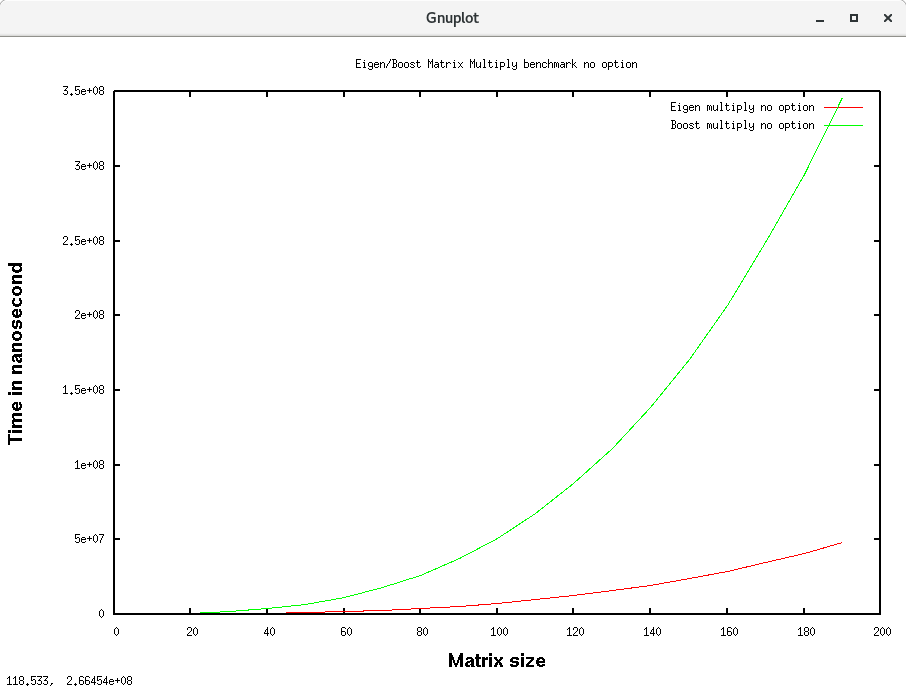
\includegraphics[width=\linewidth]{benchmark_multiply.png}
        \caption{Matrix multiply benchmark with no compile options }
        \label{Matrix multiply benchmark}
    \end{figure}

    One can graphicaly see that Eigen performance is a lot better than Boost about matrix multiplication, even with a small matrix size. This is shown here with no compile options but has also been checked with the aforehead mentionned options.
    
    \newpage
    Now let's see what is the effect of the different compile options one both library with \ref{Eigen Matrix multiply benchmark} and \ref{Boost Matrix multiply benchmark}
  \begin{figure}[h]
    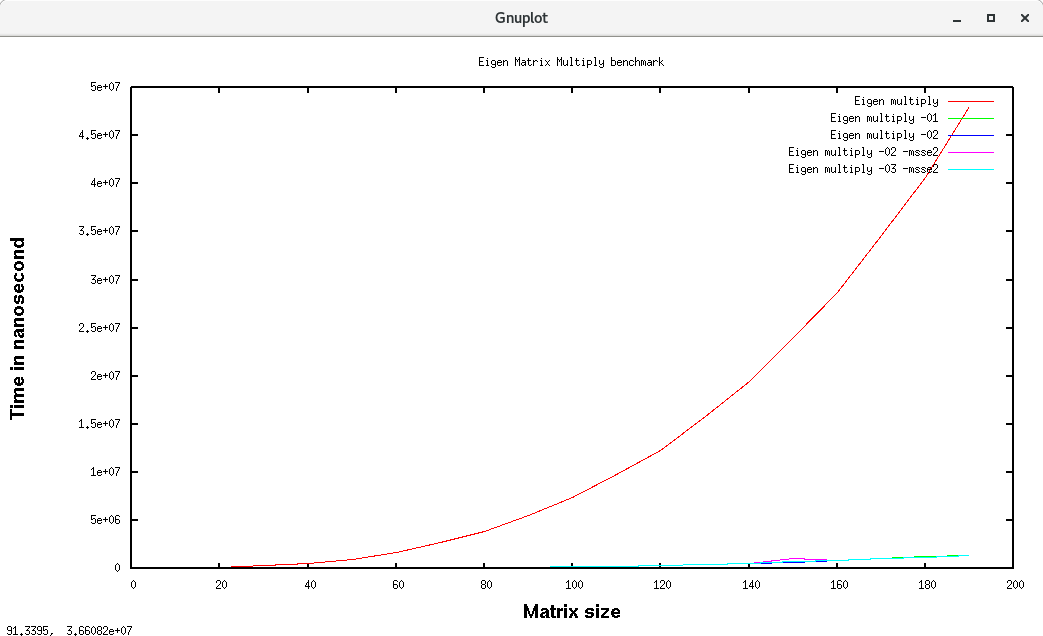
\includegraphics[width=442px]{benchmark_eigen_compilation_option.png}
    \caption{Eigen Matrix multiply benchmark with different compilation options}
    \label{Eigen Matrix multiply benchmark}
  \end{figure}
  
  \begin{figure}[h!]
    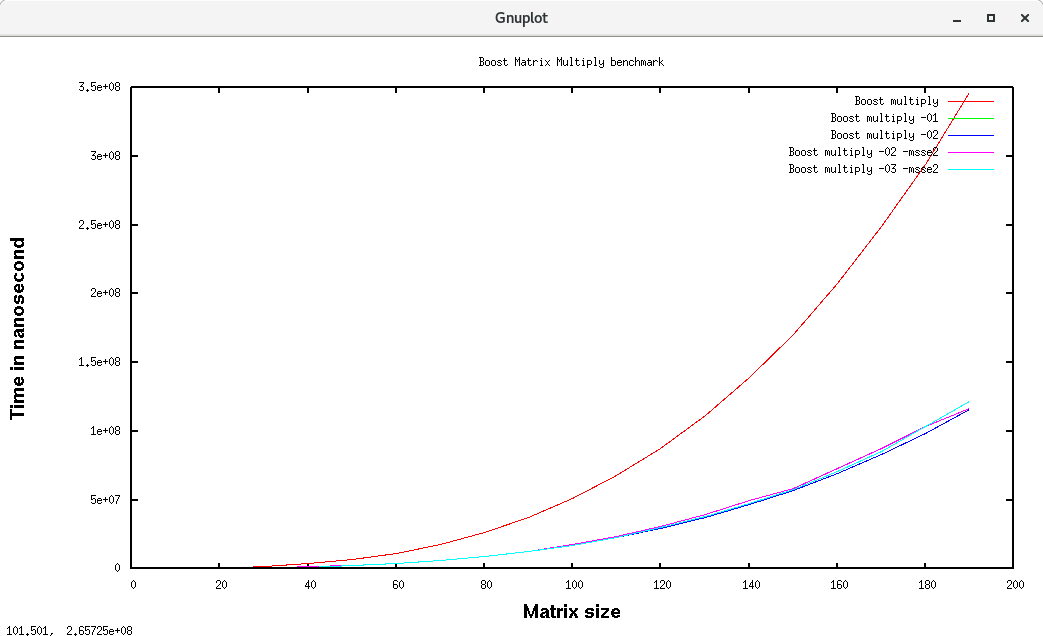
\includegraphics[width=442px]{benchmark_Boost_compilation_option.png}
    \caption{Boost Matrix multiply benchmark with different compilation options}
    \label{Boost Matrix multiply benchmark}
  \end{figure}
  
  
  
    One can observe for both library a great performance improvement between without (red line) or with (other color lines) compile options. But the performance gain over all different levels of optimisation during compilation seems negligible. Note also that the compilation optimisation give much better result for Eigen than for Boost.
    The choice of doing further optimisations during compilation is a trade-off. The higher the optimisation level is, the slower will be the compilation, but the faster will be the execution. 
    
\hspace{20px}
    
    Now we will be interested in affecting multiple cpu to the matrix multiplication task. Our lab computer have 4 cpu, so we will affect 4 cpu to the multiplication task. We do this using the command 'taskset -c 0,1,2,3 ./matrixMultiplication'. In figure \ref{cpu} we find performance comparison using 1 or 4 on the eigen matrix multiplication. Notice that for this plot we have used the "-O3 -msse2" compile options for both curve.

    \begin{figure}[h!]
    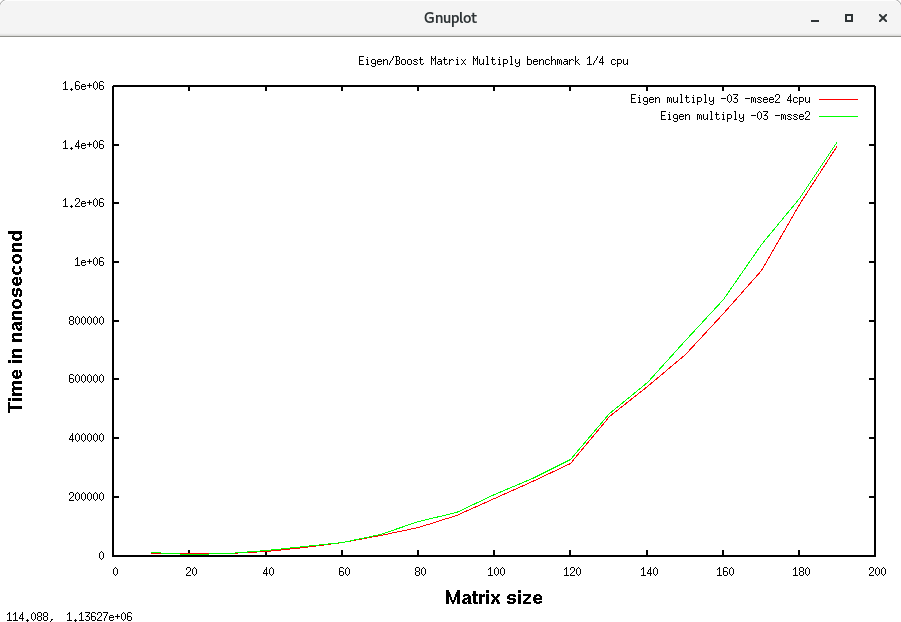
\includegraphics[width=\linewidth]{benchmark_eigen_cpu.png}
    \caption{Eigen Matrix multiply benchmark using 1 and 4 cpu}
    \label{cpu}
    \end{figure}
    One can notice that the time improvement of the 4 cpu affectation is very low for this example. It's maybe due to the fact that the eigen matrix multiplication is not parallelised. Therefore one single thread doing the computation on one cpu. So there is no point to affect more than one cpu to this task. 
    
\newpage

\section{Conclusion}
This practical gave us the chance to improve our knowledge on \textbf{CMake} and see how it facilitates the compilation and linking process by creating a Makefile for us.
In the comparison of the two libraries, Eigen clearly surpass Boost. More important is the effect of the compile options, which at the cost of a slightly longer compilation, brings huge improvement in the matrix multiplication operations.
A continuation track would be to compare the performance of the two libraries to solve linear systems (at least in mean square).


%----------------------------------------------------------------------------------------
%	BIBLIOGRAPHY
%----------------------------------------------------------------------------------------

\renewcommand{\refname}{\spacedlowsmallcaps{References}} % For modifying the bibliography heading

\bibliographystyle{plainnat}
\bibliography{bib/sample.bib} % The file containing the bibliography
%----------------------------------------------------------------------------------------

\end{document}pierre.blancfat@gmail.com